\documentclass[11pt, a4paper, spanish]{article}

%%%%%%%%%% COMIENZO DEL PREAMBULO %%%%%%%%%%

%Info sobre este documento
\author{Martin Cammi}
\title{Trabajo Pr'actico de Ingenier'ia del software I}

%\usepackage{infostyle}                                                  % provee un look & feel similar a un documento Word
\usepackage[top=2.5cm, bottom=2.5cm, left=2.5cm, right=2.5cm]{geometry}  % m\'argenes
\usepackage[ansinew]{inputenc}                                           % permite que los acentos del estilo \'a\'e\'i\'o\'u salgan joya
\usepackage[spanish, activeacute]{babel}                                 % idioma espa\~{n}ol, acentos f\'aciles y deletreo de palabras
\usepackage{indentfirst}                                                 % permite indentar un parrafo a mano
\usepackage{caratula}                                                    % incluye caratula est\'andar
\usepackage{graphicx}                                                    % permite insertar gr\'aficos
\usepackage{color}                                                       % permite el uso de colores en el documento
\usepackage[pdfcreator={TexLive!, LaTeX2e con TeXnicCenter y la inteligencia de Jonathan ;-)},
			pdfauthor={Grupo 2"},
			pdftitle={Base de Datos - Trabajo practico: Campeonato Sudamericano de B\'asquet},
			pdfsubject={Trabajo Practico de Modelo de Entidad Relación},
			pdfkeywords={MER, MR},
			pdfstartview=FitH,            % Fits the width of the page to the window
			bookmarksnumbered,            % los bookmarks numerados se ven mejor...
			colorlinks,                   % links con bellos colores
			linkcolor=magenta]            % permite cambiar el color de los links
			{hyperref}                    % Permite jugar con algunas cosas que aparecer\'an en el PDF final
\usepackage{hyperref}
\usepackage{rotating}
\usepackage{ulem}


%\selectlanguage{spanish}

\linespread{1.3}                    % interlineado equivalente al 1.5 l\'ineas de Word...
\pagestyle{myheadings}              %encabezado personalizable con \markboth{}{}
\markboth{}{Campeonato Sudamericano de B\'asquet. (Cammi, De Sousa, M\'endez, Serapio) }
\headsep = 30pt                     % separaci\'on entre encabezado y comienzo del p\'arrafo

%\addtolength{\oddsidemargin}{-2cm}	% configuracion IDEAL!!!
%\addtolength{\textwidth}{4cm}
%\addtolength{\textheight}{2cm}

% macro 'todo' para To-Do's
\def\todo#1{\textcolor{red}{#1}}

% Macro 'borde' para un texto con borde
\newsavebox{\fmbox}
\newenvironment{borde}[1]
{\begin{lrbox}{\fmbox}\begin{minipage}{#1}}
{\end{minipage}\end{lrbox}\fbox{\usebox{\fmbox}}\\[10pt]}

%%%%%%%%%% FIN DEL PREAMBULO %%%%%%%%%%

\begin{document}

\materia{Base de Datos}
\submateria{Segundo Cuatrimestre de 2012}
\titulo{Trabajo pr\'actico 1}
\subtitulo{Campeonato Sudamericano de B\'asquet.}
\grupo{Grupo 2}

\integrante{Cammi, Mart\'in}{676/02}{martincammi@gmail.com}
\integrante{De Sousa, Mariano}{389/08}{marian\_sabianaa@hotmail.com}
\integrante{M\'endez, Gonz\'alo}{843/04}{gemm83@hotmail.com}
\integrante{Serapio, Noelia}{871/03}{noeliaserapio@gmail.com}

\maketitle

\thispagestyle{empty}

\tableofcontents

\newpage

% Conviene poner las secciones como diferentes archivos,
% sobre todo cuando se trabaja en equipo.
% Es m\'as f\'acil para sincronizar mediante control de versiones.
%\input{Introducci\'on}


% BEGIN Ejemplos de uso

	%\section{Una secci\'on}
	%\label{sec:unaSeccion}
	%Hola! Soy una Secci\'on
	%	\subsection{Una subsecci\'on}
	%		Y yo soy una subsecci\'on!!!
	%		\subsubsection{Una subsubsecci\'on}
	%			Y yo soy una sub-subsecci\'on!!!
	%			\paragraph{Un p\'arrafo\\}
	%				Y yo soy un p\'arrafo, porque no hay mas sub-sub-sub-subsecciones!!!

	%\section{Otra secci\'on}
	%	Como pudimos ver en la secci\'on \ref{sec:unaSeccion}, esto es una demo de una referencia a una secci\'on.
	
	%	Tambi\'en podemos hacer referencia a la p\'agina de la secci\'on:\\[10pt]
	
		% Ejemplo de uso de un borde (falta pulir para que no tire un warning!)
	%	\begin{borde}{0.98\textwidth}
	%		En la p\'agina \pageref{sec:unaSeccion}, hay una secci\'on pilla...
	%	\end{borde}

% END Ejemplos de uso

\newpage
\section{Tecnolog\'ias utilizadas}
Hemos utilizado para la confecci\'on del trabajo pr\'actico el motor de base de datos Mysql

\newpage
	
\section{Modelo Entidad-Relacion}

	%\begin{sidewaysfigure}
%	\begin{center}
%		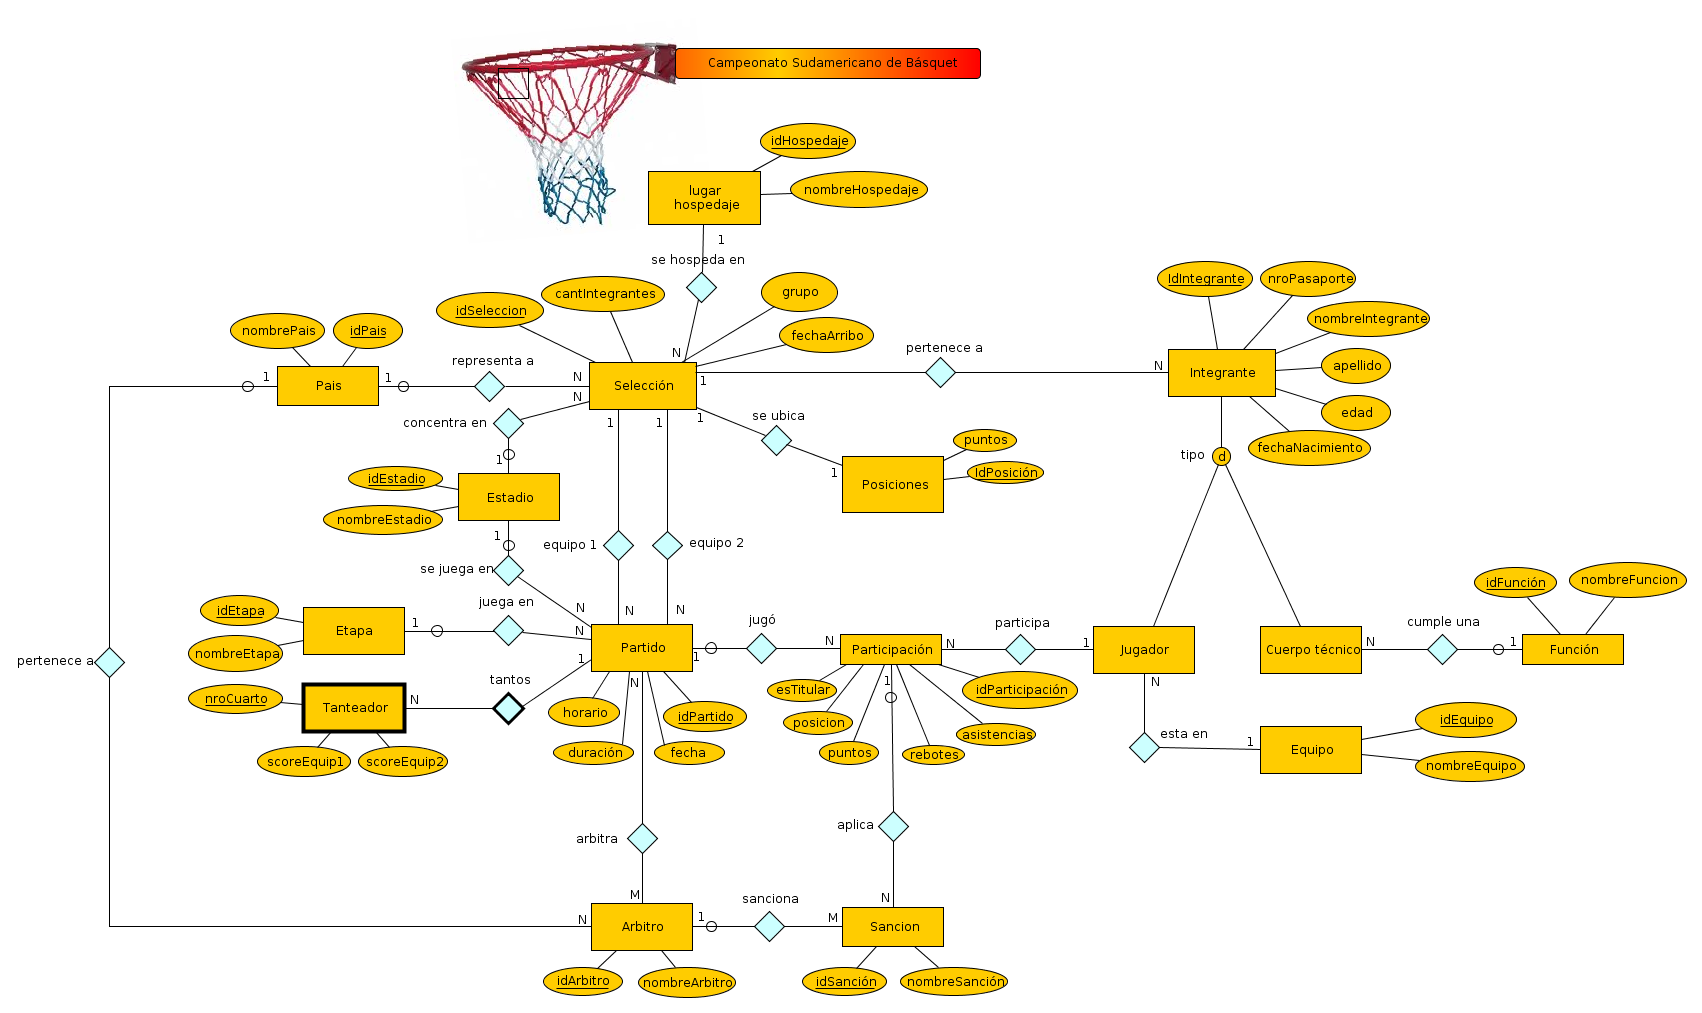
\includegraphics[scale=0.35]{diagramas/DiagramaMER.png}\\
%	\end{center}
	%\end{sidewaysfigure}
	
%\begin{figure}[h]
%\centering
%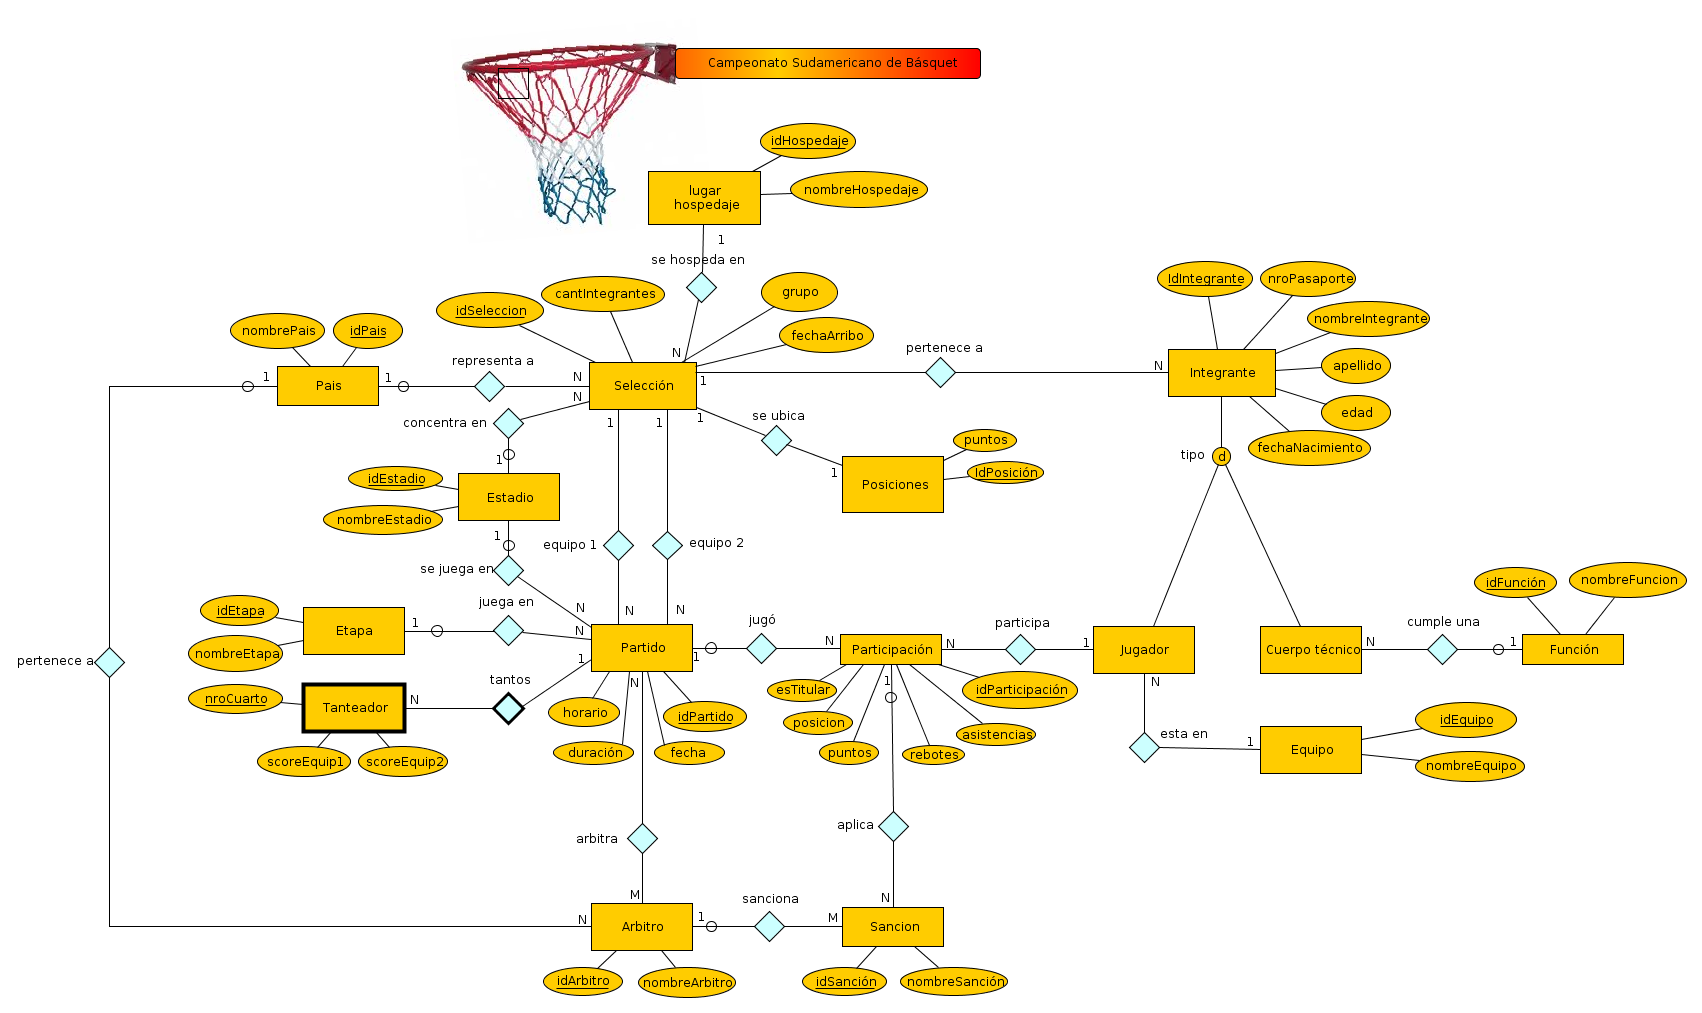
\includegraphics[width=3cm,height=3cm]{diagramas/DiagramaMER.png}
%\end{figure}
%\newpage 

\section{Modelo Logico Relacional}

\subsection{Entidad Selecci'on}
\textbf{SELECCION}(\underline{idSeleccion}, \dashuline{hospedaHospedaje}, \dashuline{representaPais}, \dashuline{concentraEstadio}, \dashuline{ubicaPosicion}, cantIntegrantes, fechaArribo, grupo)\\

PK = \{ (idSeleccion) \}\\
\indent{CC = \{ (idSeleccion) \}}\\
\indent{FK = \{ (hospedaHospedaje), (representaPais), (concentraEstadio), (ubicaPosicion) \}}\\

\noindent{ \textbf{References:}}

SELECCION.hospedaHospedaje debe estar en LUGARHOSPEDAJE.idHospedaje.\\ 
\indent{SELECCION.representaPais debe estar en PAIS.idPais.}\\
\indent{SELECCION.concentraEstadio debe estar en ESTADIO.idEstadio.}\\
\indent{SELECCION.ubicaPosicion debe estar en POSICION.idPosicion.}\\
\indent{SELECCION.idSeleccion debe estar en INTEGRANTE.perteneceSeleccion.} \\
\indent{SELECCION.idSeleccion debe estar en PARTIDO.equipoSeleccion1.} \\
\indent{SELECCION.idSeleccion debe estar en PARTIDO.equipoSeleccion2.} \\

\indent{SELECCION.hospedaHospedaje no puede ser nulo.}\\
\indent{SELECCION.representaPais no puede ser nulo.}\\
\indent{SELECCION.concentraEstadio no puede ser nulo.}\\
\indent{SELECCION.ubicaPosicion no puede ser nulo.}\\


\noindent{ \textbf{Constraints:}}

\indent{SELECCION.grupo $==$ ``A`` no puede repetirse m'as de 4 veces.}\\
\indent{SELECCION.grupo $==$ ``B`` no puede repetirse m'as de 4 veces.}\\
\indent{SELECCION.grupo solo puede ser ``A`` o ``B``.}\\
\indent{SELECCION.fechaArribo $<=$ PARTIDO.fecha.}\\
\indent{$\#$ SELECCION.cantIntegrantes debe ser igual a la cantidad de integrantes relacionados.}


\subsection{Entidad Posici'on}
\textbf{POSICION}(\underline{idPosicion}, puntos, partidosJugados, partidosGanados, partidosPerdidos, tantosAFavor, tantosEnContra)\\

PK = \{ (idPosicion) \} \\
\indent{CC = \{ (idPosicion) \}} \\
\indent{FK = \{\}} \\

\noindent{ \textbf{References:}}

\indent{POSICION.idPosicion debe estar en SELECCION.ubicaPosicion.}\\

\noindent{ \textbf{Constraints:}}

\indent{POSICION.puntos $>=$ 0.}\\
\indent{POSICION.partidosJugados $>=$ 0.}\\
\indent{POSICION.partidosGanados $>=$ 0.}\\
\indent{POSICION.partidosPerdidos $>=$ 0.}\\
\indent{POSICION.partidosJugados $==$ POSICION.partidosGanados  +  POSICION.partidosPerdidos.}\\
\indent{POSICION.tantosAFavor $>=$ 0.}\\
\indent{POSICION.tantosEnContra $>=$ 0.}

\subsection{Entidad LugarHospedaje}
\textbf{LUGARHOSPEDAJE}(\underline{idHospedaje}, nombreHospedaje)\\

PK = \{ (idHospedaje) \}\\
\indent{CC = \{ (idHospedaje) \}}\\
\indent{FK = \{\}}\\

\noindent{ \textbf{References:}}

LUGARHOSPEDAJE.idHospedaje debe estar en SELECCION.hospedaHospedaje. \\

\noindent{ \textbf{Constraints:}}

\indent{Ninguna.}

\subsection{Entidad Pa'is}
\textbf{PAIS}(\underline{idPais}, nombrePais)\\

PK = \{ (idPais) \}\\
\indent{CC = \{ (idPais) \}}\\
\indent{FK = \{\}}\\

\noindent{ \textbf{References:}}

\indent{PAIS.idPais  puede no estar en SELECCION.representaPais.}\\
\indent{PAIS.idPais  puede no estar en ARBITRO.pertenecePais.}\\

\noindent{ \textbf{Constraints:}}

\indent{Ninguna.}

\subsection{Entidad Integrante}
\textbf{INTEGRANTE}(\underline{idIntegrante}, \dashuline{perteneceSeleccion}, nroPasaporte, nombreIntegrante, apellido, fechaNacimiento,tipoIntegrante)\\

PK = \{ (idIntegrante) \} \\
\indent{CC = \{ (idIntegrante), (nroPasaporte) \}} \\
\indent{FK = \{ (perteneceSeleccion) \}} \\

\noindent{ \textbf{References:}}

\indent{INTEGRANTE.perteneceSeleccion debe estar en SELECCION.idSeleccion.} \\
\indent{INTEGRANTE.idIntegrante debe estar en JUGADOR.idJugador o (exclusivo) CUERPOTECNICO.idCuerpoTecnico.} \\

\indent{INTEGRANTE.perteneceSeleccion no puede ser nulo.} \\

\noindent{ \textbf{Constraints:}}

\indent{INTEGRANTE.tipoIntegrante IN \{ ``Jugador``, ``CuerpoTecnico`` \} .} \\
\indent{A\~{N}O(SYSDATE) $-$ A\~{N}O(INTEGRANTE.fechaNacimiento) $>=$ 18.} 


\subsection{Entidad Jugador}
\textbf{JUGADOR}(\underline{\dashuline{idJugador}}, \dashuline{estaEnEquipo})\\

PK = \{ (idJugador) \} \\
\indent{CC = \{ (idJugador) \} }\\
\indent{FK = \{ (estaEnEquipo), (idJugador) \} }\\

\noindent{ \textbf{References:}}

\indent{JUGADOR.idJugador debe estar en INTEGRANTE.idIntegrante.} \\
\indent{JUGADOR.estaEnEquipo debe estar en  EQUIPO.idEquipo.} \\
\indent{JUGADOR.idJugador debe estar en PARTICIPACION.participaJugador.} \\


\indent{JUGADOR.estaEnEquipo no puede ser nulo.} \\

\noindent{ \textbf{Constraints:}}

\indent{Por jugador, tiene que haber una sola participaci'on en un partido.}

\subsection{Entidad CuerpoT'ecnico}
\textbf{CUERPOTECNICO}(\underline{\dashuline{idCuerpoTecnico}}, \dashuline{cumpleFuncion}) \\

PK = \{ (idCuerpoTecnico) \} \\
\indent{CC = \{ (idCuerpoTecnico) \} } \\
\indent{FK = \{ (cumpleFuncion), (idCuerpoTecnico) \} } \\

\noindent{ \textbf{References:}}

\indent{CUERPOTECNICO.idCuerpoTecnico debe estar en INTEGRANTE.idIntegrante.} \\
\indent{CUERPOTECNICO.cumpleFuncion debe estar en FUNCION.idFuncion.} \\

\indent{CUERPOTECNICO.cumpleFuncion no puede ser nulo.} \\

\noindent{ \textbf{Constraints:}}

\indent{Ninguna.}

\subsection{Entidad Funci'on}
\textbf{FUNCION}(\underline{idFuncion}, nombreFuncion) \\

PK = \{ (idFuncion) \} \\
\indent{CC = \{ (idFuncion) \} }  \\
\indent{FK = \{\} } \\

\noindent{ \textbf{References:}}

\indent{FUNCION.idFuncion puede no estar en CUERPOTECNICO.cumpleFuncion. \\

\noindent{ \textbf{Constraints:}}

\indent{Ninguna.}

\subsection{Entidad Equipo}
\textbf{EQUIPO}(\underline{idEquipo}, nombreEquipo) \\

PK = \{ (idEquipo) \} \\
\indent{CC = \{ (idEquipo) \} }\\
\indent{FK = \{\} }\\

\noindent{ \textbf{References:}}

\indent{EQUIPO.idEquipo debe estar en JUGADOR.estaEnEquipo.} \\

\noindent{ \textbf{Constraints:}}

\indent{Ninguna}

\subsection{Entidad Partido}
\textbf{PARTIDO}(\underline{idPartido}, \dashuline{juegaEnEtapa}, \dashuline{equipoSeleccion1}, \dashuline{equipoSeleccion2}, \dashuline{juegaEnEstadio}, duracion, fecha, horario) \\

PK = \{ (idPartido) \} \\
\indent{CC = \{ (idPartido) \} \\
\indent{FK = \{ (juegaEnEtapa), (equipoSeleccion1), (equipoSeleccion2), (juegaEnEstadio) \} \\

\noindent{ \textbf{References:}}

\indent{PARTIDO.juegaEnEtapa debe estar en ETAPA.idEtapa.} \\
\indent{PARTIDO.equipoSeleccion1 debe estar en SELECCION.idSeleccion.} \\
\indent{PARTIDO.equipoSeleccion2 debe estar en SELECCION.idSeleccion.} \\
\indent{PARTIDO.juegaEnEstadio debe estar en ESTADIO.idEstadio.} \\
\indent{PARTIDO.idPartido debe estar en ARBITRA.idPartidoArb.} \\ 
\indent{PARTIDO.idPartido puede no estar en PARTICIPACION.jugoPartido.} \\
\indent{PARTIDO.idPartido debe estar en TANTEADOR.idPartido.} \\

\indent{PARTIDO.juegaEnEtapa no puede ser nulo.} \\
\indent{PARTIDO.equipoSeleccion1 no puede ser nulo.} \\
\indent{PARTIDO.equipoSeleccion2 no puede ser nulo.} \\
\indent{PARTIDO.juegaEnEstado no puede ser nulo.} \\

\noindent{ \textbf{Constraints:}}

\indent{PARTIDO.equipoSeleccion1 $<>$ PARTIDO.equipoSeleccion2.} \\
\indent{Si PARTIDO.juegaEnEtapa $==$ ``FASE\_GRUPOS`` $\Rightarrow$  PARTIDO.equipoSeleccion1.grupo $==$ PARTIDO.equipoSeleccion2.grupo.} \\
\indent{Si PARTIDO.juegaEnEtapa $==$ ``FASE\_GRUPOS`` $\Rightarrow$  $\#$ PARTIDO $<=$ 6.} \\
\indent{Si PARTIDO.juegaEnEtapa $==$ ``5TO\_PUESTO`` $\Rightarrow$  $\#$ PARTIDO $<$= 1.} \\
\indent{Si PARTIDO.juegaEnEtapa $==$ ``3ER\_PUESTO`` $\Rightarrow$  $\#$ PARTIDO $<=$ 1.} \\
\indent{Si PARTIDO.juegaEnEtapa $==$ ``SEMIFINAL`` $\Rightarrow$  $\#$ PARTIDO $<=$ 2.} \\
\indent{Si PARTIDO.juegaEnEtapa $==$ ``FINAL`` $\Rightarrow$  $\#$ PARTIDO $<=$ 1.} \\
\indent{No puede haber dos partidos en un mismo horario.} \\
\indent{Validar que al insertar un partido, esten todos los anteriores de fase.} \\
\indent{Las fechas de los partidos tienen que estar ordenado por la etapa (FASE\_GRUPO $<$ 5TO\_PUESTO $<$ SEMIFINAL $<$ 3ER\_PUESTO $<$ FINAL).} \\
\indent{La duraci'on de los partidos tiene que ser $>$ 0.} \\
\indent{La hora del partido tiene que estar entre 0 y 23.} \\
\indent{Dos equipos no pueden enfrentarse en la misma etapa dos veces.} \\

\subsection{Entidad Estadio}
\textbf{ESTADIO}(\underline{idEstadio}, nombreEstadio) \\

PK = \{ (idEstadio) \} \\
\indent{CC = \{ (idEstadio) \} }\\
\indent{FK = \{\} } \\

\noindent{ \textbf{References:}}

ESTADIO.idEstadio puede no estar en PARTIDO.juegaEnEstadio. \\
ESTADIO.idEstadio puede no estar en SELECCION.concentraEstadio. \\

\noindent{ \textbf{Constraints:}}

\indent{Ninguna.}

\subsection{Entidad Etapa}

\textbf{ETAPA}(\underline{idEtapa}, nombreEtapa)

PK = \{ (idEtapa) \} \\
\indent{CC = \{ (idEtapa) (nombreEtapa) \} } \\
\indent{FK = \{\} } \\

\noindent{ \textbf{References:}}

ETAPA.idEtapa puede no estar en PARTIDO.juegaEnEtapa. \\

\noindent{ \textbf{Constraints:}}

ETAPA.nombreEtapa debe ser o bien FASE\_GRUPOS o 5TO\_PUESTO, o 3ER\_PUESTO o SEMIFINAL, o FINAL. 

\subsection{Entidad Tanteador}
\textbf{TANTEADOR}(\underline{nroCuarto}, \underline{\dashuline{idPartido}}, scoreEquip1, scoreEquip2)

PK = \{ (nroCuatro, idPartido) \} \\
\indent{CC = \{ (nroCuarto,idPartido) \} } \\
\indent{FK = \{ (idPartido) \} } \\

\noindent{ \textbf{References:}}

TANTEADOR.idPartido debe estar en PARTIDO.idPartido. \\

\indent{TANTEADOR.idPartido no puede ser nulo. \\

\noindent{ \textbf{Constraints:}}

Los valores posibles de TANTEADOR.nroCuatro son \{1 ,2 , 3, 4\}. \\ 
\indent{TANTEADOR.scoreEquip1 $>=$ 0.} \\  
\indent{TANTEADOR.scoreEquip2 $>=$ 0.} \\ 
\indent{Si TANTEADOR.nroCuarto $==$ 4 $\Rightarrow$ TANTEADOR.scoreEquip1 $<>$ TANTEADOR.scoreEquip2 (no hay empates).} \\   

\noindent{ \textbf{Constraints Adicionales:}}

\indent{TANTEADOR.nroCuarto no puede aparecer m'as de 4 veces por  TANTEADOR.idPartido (el tanteador se genera con los 4 cuartos cuando se genera un partido). }  

\subsection{Entidad Arbitro}
\textbf{ARBITRO}(\underline{idArbitro}, \dashuline{pertenecePais}, nombreArbitro)

PK = \{ (idArbitro) \} \\
\indent{CC = \{ (idArbitro) \} } \\
\indent{FK = { (pertenecePais) \} } \\

\noindent{ \textbf{References:}}

\indent{ARBITRO.pertenecePais debe estar en PAIS.idPais.} \\
\indent{ARBITRO.idArbitro debe estar en ARBITRA.idArbitroArb.} \\ 
\indent{ARBITRO.idArbitro puede no estar en SANCION.sancionadaPorArbitro.} \\ 

\indent{ARBITRO.pertenecePais no puede ser nulo.} \\

\noindent{ \textbf{Constraints:}}

\indent{Ninguna.} \\

\noindent{ \textbf{Constraints Adicionales:}} 

Un 'arbitro no puede dirigir un partido si: 
\begin{itemize}
\item Dirigi'o a alguno de los equipos 2 o m'as veces, y en todos los partidos el equipo obtuvo el mismo resultado (gan'o o perdi'o, no hay empate).
\item Dirigi'o una sola vez a cada equipo con resultados opuestos.        
\item Est'a asignado a dirigir un partido en la misma fecha.    
\end{itemize}

\subsection{Entidad Arbitra}
\textbf{ARBITRA}(\underline{\dashuline{idArbitroArb}}, \underline{\dashuline{idPartidoArb}})

PK = \{ (idArbitroArb, idPartidoArb) \} \\
\indent{CC = \{ (idArbitroArb, idPartidoArb) \} } \\
\indent{FK = \{ (idArbitroArb), (idPartidoArb) \} } \\

\noindent{ \textbf{References:}}

ARBITRA.idArbitroArb debe estar en ARBITRO.idArbitro. } \\
\indent{ARBITRA.idPartidoArb debe estar en PARTIDO.idPartido. } \\

\noindent{ \textbf{Constraints:}}

(ARBITRO.idArbitro $==$ ARBITRA.idArbitroArb) and (ARBITRA.idPartidoArb $==$ PARTIDO.idPartido) $\Rightarrow$  (ARBITRO.pertenecePais $<>$ PARTIDO.seleccionEquipo1.representaPais and ARBITRO.pertenecePais $<>$ PARTIDO.seleccionEquipo2.representaPais). 

\subsection{Entidad Participaci'on}
\textbf{PARTICIPACION}(\underline{idParticipacion}, \dashuline{jugoPartido}, \dashuline{participaJugador}, asistencias, rebotes, posicion, puntos, esTitular)

PK = \{ (idParticipacion) \} \\
\indent{CC = \{ (idParticipacion) \} } \\
\indent{FK = \{ (jugoPartido), (participaJugador) \} } \\

\noindent{ \textbf{References:}}

PARTICIPACION.jugoPartido debe estar en PARTIDO.idPartido. \\
\indent{PARTICIPACION.participaJugador debe estar en JUGADOR.idIntegrante.} \\
\indent{PARTICIPACION.idParticipacion puede no estar en SANCION.aplicaParticipacion.} \\
\indent{PARTICIPACION.posicion puede ser o bien BASE o ESCOLTA o ALERO o ALA-PIVOT o PIVOT o nulo.} \\

\indent{PARTICIPACION.jugoPartido no puede ser nulo.} \\
\indent{PARTICIPACION.participaJugador no puede ser nulo.} \\

\noindent{ \textbf{Constraints:}}

PARTICIPACION.jugoPartido.equipoSeleccion1 puede aparecer a lo sumo 5 veces con PARTICIPACION.esTitular $==$ true. \\
\indent{PARTICIPACION.jugoPartido.equipoSeleccion2 puede aparecer a lo sumo 5 veces con PARTICIPACION.esTitular $==$ true.} \\
\indent{No puede haber dos PARTICIPACION.participaJugador tal que PARTICIPACION.esTitular $==$ true y  PARTICIPACION.participaJugador.IdIntegrante.perteneceSeleccion  sean iguales y PARTICIPACION.posicion sean iguales.} \\
\indent{PARTICIPACION.rebotes $>=$ 0.} \\
\indent{PARTICIPACION.asistencias $>=$ 0.} \\ 
\indent{PARTICIPACION.puntos $>=$ 0.}  \\
\indent{Si PARTICIPACION.esTitular $==$ false $\Rightarrow$ PARTICIPACION.posicion is null.}   

\subsection{Entidad Sanci'on}
\textbf{SANCION}(\underline{idSancion}, \dashuline{aplicaParticipacion}, \dashuline{sancionadaPorArbitro}, \dashuline{esDeTipo})

PK = \{ (idSancion) \} \\
\indent{CC = \{ (idSancion) \} } \\
\indent{FK = \{ (aplicaParticipacion) , (sancionadaPorArbitro), (esDeTipo) \} } \\

\noindent{ \textbf{References:}}

SANCION.aplicaParticipacion debe estar en PARTICIPACION.idParticipacion.} \\
\indent{SANCION.sancionadaPorArbitro debe estar en ARBITRO.idArbitro.} \\
\indent{SANCION.esDeTipo debe estar en TIPOSANCION.idTipoSancion.} \\

\indent{SANCION.aplicaParticipacion no puede ser nulo.} \\
\indent{SANCION.sancionadaPorArbitro no puede ser nulo.} \\
\indent{SANCION.esDeTipo no puede ser nulo.} \\

\noindent{ \textbf{Constraints:}}

\indent{ARBITRA.idArbitroArb $==$ SANCION.sancionadaPorArbitro  and ARBITRA.idPartidoArb $==$  SANCION.aplicaParticipacion.jugoPartido.} 

\subsection{Entidad TipoSanci'on}
\textbf{TIPOSANCION}(\underline{idTipoSancion}, nombreSancion)
PK = \{ (idTipoSancion) \} \\
\indent{CC = \{ (idTipoSancion) \} } \\
\indent{FK = \{\} } \\

\noindent{ \textbf{References:}}

\indent{TIPOSANCION.idTipoSancion puede no estar en SANCION.esDeTipo.} \\

\noindent{ \textbf{Constraints:}}

\indent{Ninguna.}



 













\newpage 
\section{Supuestos asumidos}
Asumimos que s'olo vamos a guardar los hospedajes que nos indiquen de los jugadores, no otros. \\
\indent{Asumimos que s'olo vamos a querer guardar los equipos en que jueguen los jugadores de la selecci'on.}

\newpage 
\section{Dise\~{n}o f\'isico}
Detalle grafico o escrito de las tablas de mysql

\newpage 
\section{Restricciones adicionales al modelo}
Las 1000 restricciones que pusimos.

\newpage 
\section{Breakers}

Los breakers son sentencias de inserts dise\~{n}adas espec\'ificamente para poner a prueba las restricciones del modelo.
El archivo breakers.sql permite ejecutarlas y ver como todas ellas se verifican.

\newpage 
\section{Triggers y Store Procedures de restricciones}


\newpage 
\section{Datos de prueba}
Imagen de datos.sql y el fixture de los partidos con los puntajes

Todo el trabajo pr\'actico cuenta con 

\end{document}
